\documentclass{beamer}

\usepackage{amsmath}
\usepackage[utf8]{inputenc}
\usepackage{listings}
\usepackage{ulem}
\usepackage{xcolor}

\lstdefinelanguage{scala}{
  morekeywords={
    abstract
  , case
  , catch
  , class
  , copy
  , def
  , do
  , else
  , extends
  , false
  , final
  , finally
  , for
  , if
  , implicit
  , import
  , match
  , mixin
  , new
  , null
  , object
  , override
  , package
  , private
  , protected
  , requires
  , return
  , sealed
  , super
  , this
  , throw
  , trait
  , true
  , try
  , type
  , val
  , var
  , while
  , with
  , yield
  }
, sensitive=true
, morecomment=[l]{//}
, morecomment=[n]{/*}{*/}
, morestring=[b]"
, morestring=[b]'
, morestring=[b]"""
}

% set font with bold
\renewcommand{\ttdefault}{pcr}

\lstset{
  language=Scala
, tabsize=2
, basicstyle=\ttfamily
, keywordstyle=\color{darkgray}\bfseries
, breaklines=true
}


\usetheme{RBE}
\usecolortheme{RBE}
\setbeamercovered{transparent}
\setbeamertemplate{headline}{
  \begin{beamercolorbox}{section in head/foot}
    \vskip2pt\insertnavigation{\paperwidth}\vskip2pt
  \end{beamercolorbox}
}

\setbeamertemplate{footline}{}
\setbeamertemplate{navigation symbols}{}

\xdefinecolor{darkgreen}{rgb}{0,0.35,0}
\xdefinecolor{tomorrowcomment}{HTML}{8e908c}
\xdefinecolor{tomorrowred}{HTML}{c82829}

\xdefinecolor{tomorrowblue}{HTML}{4271ae}
\xdefinecolor{tomorrowgreen}{HTML}{718c00}
\xdefinecolor{tomorrowpurple}{HTML}{8959a8}
\xdefinecolor{tomorrowyellow}{HTML}{eab700}

\lstset{
  tabsize=2,
  basicstyle=\ttfamily,
  moredelim=**[is][\btHL]{`}{`},
  showstringspaces=false,
  breaklines=true,
  columns=fixed,
  rulesepcolor=\color{tomorrowyellow},
  numberstyle=\tiny\color{tomorroworange},
  basicstyle=\footnotesize\ttfamily,
  keywordstyle=\color{tomorrowpurple},
  stringstyle=\color{tomorrowgreen}\ttfamily,
  identifierstyle=\color{tomorrowblue},
  commentstyle=\color{tomorrowcomment},
  emphstyle=\color{tomorrowred}
}
\lstdefinestyle{language}{
  language=scala,
  basicstyle=\footnotesize\ttfamily,
  stringstyle=\color{darkgreen}\ttfamily,
  commentstyle=\color{gray}\ttfamily,
  keywordstyle=\footnotesize\color{blue}\ttfamily,
  tabsize=2,
  moredelim=**[is][\btHL]{`}{`},
  showstringspaces=false
}
\DeclareFontShape{OT1}{cmtt}{bx}{n}{<5><6><7><8><9><10><10.95><12><14.4><17.28><20.74><24.88>cmttb10}{}

\author{Ricky Elrod}

\begin{document}
\title{What is a \texttt{Lens}}
\subtitle{And why does it matter?}
\institute{Cleveland Scalawags}
\tiny{\date

}
\normalsize

\setbeamercovered{transparent}
\begin{frame}
  \titlepage
\end{frame}

\begin{frame}[fragile]
  \frametitle{First off...}
  \framesubtitle{Hi there!}
  \begin{itemize}
  \item I am a ...
    \begin{itemize}
      \item Person with a strong interest in provable software correctness.
      \item Student at Youngstown State University
      \item YSU ACM Student Chapter Vice President
      \item haskell.org infrastructure volunteer
      \item Emacs user
      \item Dog owner
      \item Pepsi drinker
    \end{itemize}
  \end{itemize}
\end{frame}

\begin{frame}[fragile]
  \frametitle{This talk}
  \begin{itemize}
    \item This talk doesn't cover the implementation of lenses.
    \item In fact, it doesn't cover a lot of things about lenses.
    \item It serves as a primer, to pique interest.
    \item It aims to demonstrate a problem and a solution.
    \item Most importantly, it aims to point you to a working implementation of the solution
    \item ...and to other Lens-related resources.
  \end{itemize}
\end{frame}

\begin{frame}[fragile]
  \frametitle{Motivation}
  \framesubtitle{Why do lenses exist?}
  \begin{itemize}
    \item We want to do programming.
    \item Specifically, we want to do \textit{functional programming}.
    \item Immutable data types are a \textit{must}.
  \end{itemize}
\end{frame}

\begin{frame}[fragile]
  \frametitle{Motivation}
  \framesubtitle{Immutable data types}
  \begin{block}{Typical data types in Scala}
    \begin{lstlisting}[language=scala]
case class City(name: String)
case class Library(name: String, mainLocation: City)
case class Branch(name: String, library: Library)
case class Book(name: String, branch: Branch)
case class BookReader(fullName: String, book: Book)
    \end{lstlisting}
  \end{block}
\end{frame}

\begin{frame}[fragile]
  \frametitle{Motivation}
  \framesubtitle{Immutable data types}
  \begin{block}{Using the structures we have made}
    \begin{lstlisting}[language=scala]
val akron = City("Akron")

val akronLibrary =
  Library("Akron-Summit County Public Library", akron)

val norton = Branch("Norton", akronLibrary)

val fpis =
  Book("Functional Programming in Scala", norton)

val borrower = BookReader("Joe Smith", fpis)
    \end{lstlisting}
    \begin{lstlisting}[language=scala]
scala> borrower
res0: BookReader = BookReader(Joe Smith,Book(Functional Programming in Scala,Branch(Norton,Library(Akron-Summit County Public Library,City(Akron)))))
    \end{lstlisting}
  \end{block}
\end{frame}

\begin{frame}[fragile]
  \frametitle{Motivation}
  \framesubtitle{Immutable data types}
  \begin{itemize}
    \item Ut oh! I've suddenly been given a new requirement.
    \item I need a function that takes a \texttt{BookReader} and gives one back with the city of the main library's location in UPPERCASE.
    \item Let's do it!
  \end{itemize}
\end{frame}

\begin{frame}[fragile]
  \frametitle{Motivation}
  \framesubtitle{Immutable data types}
  \begin{block}{Uhm...}
    \begin{lstlisting}[language=scala]
def upcaseLibrary(br: BookReader) =
  br.copy(
    book = br.book.copy(
      branch = br.book.branch.copy(
        library = br.book.branch.library.copy(
          mainLocation = br.book.branch.library.mainLocation.copy(
            name = br.book.branch.library.mainLocation.name.toUpperCase
          )
        )
      )
    )
  )
    \end{lstlisting}
  \end{block}
\end{frame}

\begin{frame}[fragile]
  \frametitle{Motivation}
  \begin{center}
    
\includegraphics[height=7cm]{img/ohgodmyeyes.png}
  \end{center}
\end{frame}

\begin{frame}[fragile]
  \frametitle{What is a lens?}
  \begin{block}{A data structure}
    \begin{lstlisting}[language=scala]
case class Lens[T, F](get: T => F, set: (T, F) => T)
    \end{lstlisting}
  \end{block}

  \begin{block}{...With a few laws}
    \begin{itemize}
      \item 0. if I get twice, I get the same answer
      \item 1. if I get, then set it back, nothing changes.
      \item 2. if I set, then get, I get what I set.
      \item 3. if I set twice then get, I get the second thing I set.
    \end{itemize}
  \end{block}
\end{frame}

\begin{frame}[fragile]
  \frametitle{Now then...}
  \begin{itemize}
    \item This concept is not new, and has been documented multiple times.
    \item Monocle is a fairly new Scala library based on this concept.
    \item Edward Kmett's "lens" library is a (very large, but very awesome) implementation for Haskell.
    \item One key concept is that lenses are composable into other lenses.
    \item Since this is a lightning talk, I will quickly show the Monocle approach.
  \end{itemize}
\end{frame}

\begin{frame}[fragile]
  \frametitle{Monocle}
  \begin{lstlisting}[language=scala]
val _name =
  SimpleLens[City, String](
    _.city, (e, c) => e.copy(city = c))

val _mainLocation =
  SimpleLens[Library, City](
    _.mainLocation, (e, c) => e.copy(mainLocation = c))

val _library =
  SimpleLens[Branch, Library](
    _.library, (e, c) => e.copy(library = c))

val _branch =
  SimpleLens[Book, Branch](
    _.branch, (e, c) => e.copy(branch = c))

val _book =
  SimpleLens[BookReader, Book](
    _.book, (e, c) => e.copy(book = c))
// ...
  \end{lstlisting}
\end{frame}

\begin{frame}[fragile]
  \frametitle{:(}
  \begin{center}
    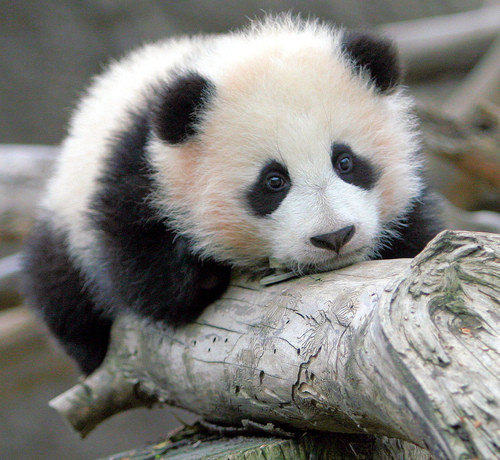
\includegraphics[height=7cm]{img/sadpanda.jpg}
  \end{center}
\end{frame}

\begin{frame}[fragile]
  \frametitle{:)}
  \begin{lstlisting}[language=scala]
import monocle.Macro._
val _name = mkLens[City, String]("name") // name is checked at compiled time to be a valid accessor
val _mainLocation = mkLens[Library, City](
  "mainLocation")
val _library = mkLens[Branch, Library]("library")
val _branch = mkLens[Book, Branch]("branch")
val _book = mkLens[BookReader, Book]("book")
// ...
  \end{lstlisting}
\end{frame}

\begin{frame}[fragile]
  \frametitle{Let's actually use it}
  \begin{lstlisting}[language=scala]
def upcaseLibrary(br: BookReader) =
  br applyLens   _book
     composeLens _branch
     composeLens _library
     composeLens _mainLocation
     composeLens _name
     modify (_.toUpperCase)
  \end{lstlisting}
\end{frame}

\begin{frame}[fragile]
  \frametitle{Sigh.}
  \begin{center}
    
\includegraphics[height=7cm]{img/sigh.png}
  \end{center}
\end{frame}

\begin{frame}[fragile]
  \frametitle{More syntactic sugar!}
  \begin{lstlisting}[language=scala]
def upcaseLibrary(br: BookReader) =
  br |->
  _book |->
  _branch |->
  _library |->
  _mainLocation |->
  name modify (_.toUpperCase)
  \end{lstlisting}
\end{frame}

\begin{frame}[fragile]
  \frametitle{Resources}
  \begin{itemize}
    \item https://github.com/julien-truffaut/Monocle/
    \item http://days2012.scala-lang.org/sites/days2012/files/morris\_lenses.pdf
    \item https://hackage.haskell.org/package/lens
  \end{itemize}
\end{frame}

\begin{frame}[fragile]
  \frametitle{Contact}
  ricky@elrod.me, @relrod6 on Twitter, ``relrod'' on Freenode IRC. Let's talk!
\end{frame}

\end{document}
